\chapter{Background}
\label{ch:background}

% http://www.ccs.neu.edu/home/will/CPP/dangling.html has a good example of a dangling pointer error leading to double delete

\section{Virtual memory}

Virtual memory is an abstraction over the physical memory available to the hardware. It's an abstraction that is typically transparent to both the applications and developers, meaning that they do not have to be aware of it, while enjoying the significant benefits. This is enabled by the hardware and operating system kernel working together in the background.

From a security and stability point of view, the biggest benefit that virtual memory provides is address space isolation: each process executes as if it was the only one running, with all of the memory visible to it belonging either to itself or the kernel. This means that a malicious or misbehaving application cannot directly access the memory of any other process, to either deliberately or due to a programming error expose secrets of the other application (such as passwords or private keys) or destabilize it by corrupting its memory.

An additional security feature is the ability to specify permission flags on individual memory pages: they can be independently made readable, writeable, and executable. For instance, all memory containing application data can be marked as readable, writeable, but not executable, while the memory pages hosting the application code can be made readable, executable, but not writeable, limiting the capabilities of attackers.

Furthermore, virtual memory allows the kernel to optimize physical memory usage by:

\begin{itemize}
	\item Compressing or swapping out (writing to hard disk) rarely used memory pages (regions) to reduce memory usage
	\item De-duplicating identical memory pages, such as those resulting from commonly used static or shared libraries
	\item Lazily allocating memory pages requested by the application
\end{itemize}

Virtual memory works by creating an artificial (virtual) address space for each process, and then mapping the appropriate regions of it to the backing physical memory. A pointer will reference a location in virtual memory, and upon access, is resolved (typically by the hardware) into a physical memory address. The granularity of the mapping is referred to as a memory page, and is typically 4096 bytes (4 kilobytes) in size. (See Figure~\ref{fig:virtual_memory}.)

\begin{figure}
	\centering
	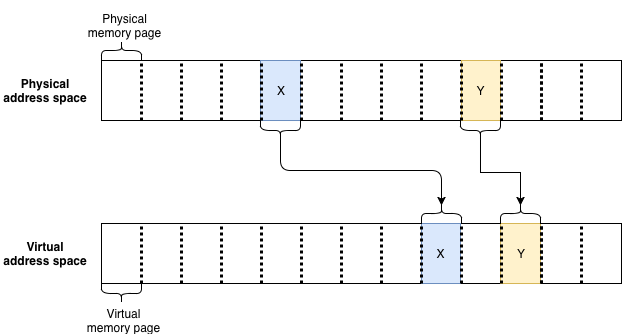
\includegraphics[width=\textwidth]{diagrams/virtual_memory.png}
	\caption{Mapping two physical memory pages X and Y to virtual memory}
	\label{fig:virtual_memory}
\end{figure}

This mapping is encoded in a data structure called the \emph{page table}. This is built up and managed by the kernel: as the application allocates and frees memory, virtual memory mappings have be created and destroyed. The representation of the page table varies depending on the architecture, but on x86-64, it can be represented as a tree, with each node an array of 512 page table entries of 8 bytes each making up a 4096 byte page table page. The root of this tree is where all virtual memory address resolution begins, and it identifies the address space. The leaf nodes are the physical memory pages that contain the application's own data.

The bits of the virtual memory address identify the page table entry to follow during address resolution. For each level of page tables, 9 bits are required to encode an index into the array of 512 entries. Each entry contains the physical memory address of the next page to traverse during the address resolution, as well as a series of bits that represent the different access permissions, such as writeable and executable. Finally, the least-significant 12 bits are used to address into the application's physical page (which is 4096 bytes) itself and so require no translation. (See Figure~\ref{fig:page_table_tree}.)

On x86-64, there are currently 4 levels of page tables, using $4 * 9 + 12 = 48$ out of the 64 available bits in the memory addresses, and limiting the size of the address space to $2^{48}$ bytes or 256 terabytes. (The size of addressable space per page table level, in reverse resolution order being: $512 * 4$ kilobytes = 2 megabytes; $512 * 2$ megabytes = 1 gigabyte; 512 gigabytes; 256 terabytes.)

\begin{figure}
	\centering
	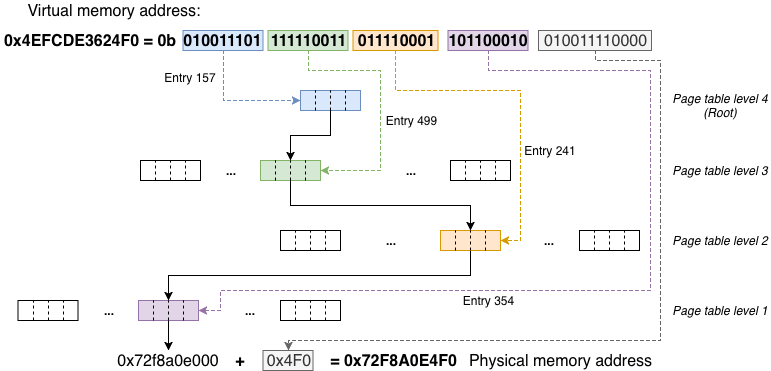
\includegraphics[width=\textwidth]{diagrams/page_table_tree.png}
	\caption{Translating a virtual memory address to physical using the page tables}
	\label{fig:page_table_tree}
\end{figure}

It's important to realize that it is possible to map a physical page into multiple virtual pages, as well as to have unmapped virtual pages. Attempting to access a virtual page (by dereferencing a pointer to it) that is not mapped -- i.e. not backed by a physical memory page -- will cause a \emph{page fault} and execution to trap inside the kernel. The kernel then can decide what to do -- for instance if it determines that the memory access was in error (an \emph{access violation}), it passes the fault on to the process which usually terminates it. On Linux this is done by raising the \texttt{SIGSEGV} signal (segmentation violation or segmentation fault) in the process, normally aborting its execution.

Other types of access violation, such as attempting to write a non-writeable page -- a page on which writing was disallowed by setting the corresponding bit in its page table entry to 0 -- or attempting to execute a non-executable page -- a page which has its no-execute bit set, a new addition in the x86-64 architecture over x86-32 -- will also trigger a page fault in the kernel the same way.

This mechanism also allows the kernel to perform memory optimizations. These are important, because (physical) memory is often a scarce resource. For example, a common scenario is that multiple running processes use the same shared library. The shared library is a single binary file on disk that is loaded into memory by multiple processes, meaning that naively the same data would be loaded into memory multiple times, taking up precious resources for no gain. The kernel can instead load the shared library into physical memory only once and then map this region into the virtual address space of each user application. Other de-duplication opportunities include static libraries that are commonly linked into applications (such as the C standard library), or the same binary executing in multiple processes.

In addition to memory de-duplication, the kernel can also choose to compress or even swap out rarely used memory. In these cases, the kernel marks the relevant page table entries as invalid, causing the hardware to trigger a page fault in the kernel if they are accessed. Upon access, instead of sending a signal to the process, the kernel restores the data by decompressing it or reading it from disk, after which it will resume the process which can continue without even being aware of what happened. Modern kernels include a large number of similar optimizations. \todo{Could probably find some citations for this}

% Thanks to Dune, Dangless has direct access to the page tables, and manipulates them using custom functions (see \textit{include/dangless/virtmem.h} and \textit{src/virtmem.c}). Upon memory allocation, Dangless forwards the allocation call to the system allocator and then reserves a new virtual page, mapping it to the same physical address as the a virtual page returned by the system allocator. This is called virtual aliasing. During deallocation, besides forwarding the call to the system allocator, Dangless unmaps the virtual alias page and overwrites the page table entry with a custom value, enabling it to recognize a would-be access through a dangling pointer.

\section{Prior art}

\todo{Oscar, etc.}

\section{Dune: light-weight process virtualization}
\label{sec:bg-dune}

Dune~\cite{dune-website} is a technology developed to enable the development of Linux applications that can run on an unmodified Linux kernel while having the ability to directly and safely (in isolation from the rest of the system) access hardware features normally reserved for the kernel (ring 0) code~\cite{dune-paper}. Importantly, while getting all the benefits of having direct access to privileged hardware features, the application still has access to the Linux host operating system's interface (system calls) and features. This means that the same process that can, for instance, directly manipulate its own interrupt descriptor table, can also call a normal \lstinline!fopen()! function (or \lstinline!open()! Linux system call) and it'll behave as expected: the system call will pass through to the host kernel.

This is achieved using hardware-assisted virtualization (Intel VT-x) on the process level, rather than on the more common machine level. Dune consists of a kernel module \texttt{dune.ko} for x86-64 Linux that initializes the virtual environment and mediates between the Dune-mode process and the host kernel, as well as a user-level library called \texttt{libdune} for setting up and managing the virtualized (guest) hardware. The two components communicate via the \lstinline!ioctl()! system call on the \texttt{/dev/dune} special device that is exposed by the kernel module. Finally, \texttt{libdune/dune.h} exposes a number of functions to help the application manage the now-accessible hardware features.

An application wishing to use Dune has to statically link to \texttt{libdune.a}, and call \lstinline!dune_init()! and \lstinline!dune_enter()! to enter Dune mode. For this to succeed, the Dune kernel mode has to be already loaded. That done, the application keeps running as before: file descriptors remain valid, system calls continue to work, and so on, except privileged hardware features also become available. This opens up drastically more efficient methods of implementing some applications, such as those utilizing garbage collection, process migration, and sandboxing untrusted code. It also enables Dangless to work efficiently.

Dune sets up the guest environment by default so it's sufficient to just make whatever modifications you need. For instance, Dune sets up system calls in the virtualized guest environment so that they are forwarded to the host kernel. It is also possible to implement your own system call handler, as many of the Dune demo applications do. Dune also sets up the virtual memory mappings. \todo{Write more about this}

\subsection{Patching Dune}

Dangless was built using ix-project's fork of Dune~\cite{dune-github-ix}, because when the Dangless project started that was more maintained and supported more recent kernel versions. However, since then, work appears to have resumed on the original Dune repository~\cite{dune-github-original}, and they now claim to be supporting Linux kernel versions 4.x.

I have patched Dune with a couple of modifications to allow Dangless to do its work. These are available in the \texttt{vendor} directory in the Dangless source code.

\texttt{dune-ix-guestppages.patch}: this maps the guest system's pagetable pages into its own virtual memory, allowing Dangless to modify them. The code for this already existed in the original implementation of Dune, but was removed at some point from the ix-project's fork.
 
\texttt{dune-ix-nosigterm.patch}: for unclear reasons, upon exiting, Dune was raising the \lstinline!SIGTERM! signal, causing the Dune process to appear to have crashed even when it exited normally. This patch disables this behaviour, without appearing to affect anything else.

\texttt{dune-ix-vmcallhooks.patch}: this is a significant patch that allows a pre- and post-hook to be registered for \lstinline!vmcall!-s. That is, any time a system call is not handled inside Dune, and is about to be forwarded to the host kernel, the pre-hook, if set, is invoked with the system call number, arguments, and return address, allowing the hook to inspect and modify them. Similarly, once the \lstinline!vmcall! returns, but before the normal code execution resumes, the post-hook is invoked, with the system call result passed to it as argument. This is critical for Dangless, and is explained in detail by Section~\ref{sec:vmcall-pointer-rewriting}.

Finally, Dangless contains a work-around for an issue in Dune which appears with allocation-heavy code. \texttt{glibc}'s default \lstinline!malloc()! implementation relies on the \lstinline!brk()! system call to perform small memory allocations (in my tests, up to 9000 bytes). After a sufficient number of \lstinline!brk()! calls, the resulting address crosses the 4 GB boundary, i.e. the memory address \texttt{0x100000000}. However, this area doesn't appear to be mapped by Dune in the embedded page table, causing an EPT violation error on access. In the Dangless source code, \texttt{testapps/memstress} can be used to trigger this bug:

\begin{verbatim}
$ cd build/testapps/memstress
$ ./memstress 1500000 9000
\end{verbatim}

To work around this, Dangless registers a post-vmcall hook, and if it detects a \lstinline!brk()! system call with a parameter above the 4 GB mark, it overwrites the system call's return code to make it appear to have failed. \texttt{glibc}'s memory allocator will then fall back to using \lstinline!mmap()! even for these smaller allocations, which will continue to work.

\subsection{Memory layout}

Dune offers two memory layouts, specified when calling \lstinline!dune_init()!: precise mappings and full mappings.
With precise mappings, Dune will consult \texttt{/proc/self/maps} for the memory regions of the so-far ordinary Linux process and map each region found there into the guest environment. With the version of Dune I was using for development, this did not appear to work correctly, and so I used full mappings for Dangless.

In full mappings, Dune creates the following mappings in the guest virtual memory:

\begin{itemize}
	\item Identity-mapping for the first 4 GB of memory: this is where the executable code and data lives, so this is also where the default \lstinline!malloc()! implementation places small memory allocations (allocated via \lstinline!brk()!)
	\item The stack memory, max 1 GB
	\item The mmap memory region, max 63 GB
	\item The static \texttt{VDSO} and \texttt{VVAR} regions
	\item Any mappings needed for the executable and libraries (code and data)
\end{itemize}

Furthermore, the Dune kernel module creates the embedded page table (EPT), the part of the Intel VT-x virtualization technology that is used for translating host virtual addresses (HVA) to guest physical addresses (GPA) and vica versa. The EPT is set up and is kept in sync with the process memory automatically, meaning that mappings are created on-demand on EPT faults, within the limits of the layout defined by Dune and described above.

Dangless makes extensive use of the knowledge of the guest memory layout, for instance for translating physical addresses (e.g. of pagetable pages) to virtual addresses.

\section{Unikernels and Rumprun}

Unikernels offer a way to specialize an operating system kernel to a specific application~\cite{unikernels-intro} -- typically a web server -- in order to reduce its image size by eliminating any features not required, reducing its attack surface, and potentially improving performance. Since 2013 the widespread use of cloud technologies have made this into a popular research topic, and gave rise to related solutions such as Docker, offering a slightly different approach. \todo{Probably some more citations here?}

---

Rumprun and rumpkernels is an example of unikernels, based on the NetBSD kernel.

When the development of Dangless began, it was initially aimed to support both Rumprun and Dune. However, Rumprun has always been more difficult to work with of the two, given how it works: compiling an application adapted specifically for this purpose from its list of supported packages, then building it into a virtual machine image together with a stripped-down version of the kernel. The application executes entirely in its own virtual machine, making testing and debugging it difficult.

Furthermore, Rumprun is built to be only used on packages that were specifically prepared for it, and the intention never was to be able to easily extend it. For instance, it defines its own strong aliases for the memory management functions \lstinline!malloc()!, \lstinline!free()!, etc. leaving no way to replace them with Dangless' functions without modifying Rumprun itself.

\todo{I think these are called unikernels - there was a discussion on these recently on HN}
\todo{Development started on rumprun, why did I end up dropping it?}
